\documentclass[../mathNotesPreamble]{subfiles}

\providecommand{\relscalefact}{1.4}
\begin{document}
\relscale{\relscalefact}
  \section{7.2: Sum and Difference Identities}

  % sum/diff sin/cos (7pi/12, pi/12, etc)
  % rewrite in terms of sin/cos
  % simplify using sum/diff
  % given sin(a)= and cos(b)=, find sin(a-b)
  % find sin(arccos(...)-arccos(...))

  \begin{defn*}[Sum and Difference formulas]
    \begin{align*}
      \sin\parens{\alpha\pm \beta}&=\sin(\alpha)\cos(\beta)\pm\cos(\alpha)\sin(\beta)\\[0.5\baselineskip]
      \cos\parens{\alpha\pm \beta}&=\cos(\alpha)\cos(\beta)\mp\sin(\alpha)\sin(\beta)
    \end{align*}
  \end{defn*}
  \begin{ex*}
    Find the exact value of the following:
    \begin{extasks}[after-item-skip=\stretch{1}](2)
      \task $\sin\parens{\dfrac{5\pi}{4}-\dfrac{\pi}{6}}$
      \task $\cos\parens{\dfrac{\pi}{3}-\dfrac{\pi}{4}}$
      \task $\sin\parens{75^\circ}$
      \task $\cos\parens{105^\circ}$
    \end{extasks}
    \vspace*{\stretch{1}}
  \end{ex*}
  \pagebreak

  \begin{ex*}
    Show the following are equivalent using the sum and difference formulas:
    \begin{extasks}[after-item-skip=\stretch{1}](2)
      \task $\sin\parens{45^\circ-30^\circ}$
      \task $\sin\parens{135^\circ-120^\circ}$
    \end{extasks}
    \vspace*{\stretch{1}}
  \end{ex*}

  \begin{ex*}
    Evaluate the following:
    \begin{extasks}[after-item-skip=\stretch{1}](1)
      \task $\sin\parens{\cos^{-1}\parens{\dfrac{1}{2}}+\sin^{-1}\parens{\dfrac{3}{5}}}$
    \end{extasks}
    \vspace*{\stretch{1}}
  \end{ex*}
  \pagebreak

  \begin{defn*}[Sum and Difference for Tangent]
    \begin{align*}
      \tan\parens{\alpha\pm \beta}&= \dfrac{\tan(\alpha) \pm \tan(\beta)}{1\mp \tan(\alpha)\tan(\beta)}
    \end{align*}
  \end{defn*}
  \begin{ex*}
    Find the exact value of the following:
    \begin{extasks}[after-item-skip=\stretch{1}](1)
      \task $\tan\parens{\dfrac{\pi}{6}+\dfrac{\pi}{4}}$
      \task $\tan\parens{\dfrac{2\pi}{3}-\dfrac{\pi}{4}}$
    \end{extasks}
    \vspace*{\stretch{1}}
  \end{ex*}
  \pagebreak

  \begin{ex*}
    Given $\sin(\alpha)=\dfrac{3}{5}$, where $0<\alpha<\dfrac{\pi}{2}$, and $\cos(\beta)=-\dfrac{5}{13}$, where $\pi<\beta< \dfrac{3\pi}{2}$, evaluate the following:
    \begin{extasks}[after-item-skip=\stretch{1}](1)
      \task $\sin(\alpha+\beta)$
      \task $\cos(\alpha+\beta)$
      \task $\tan(\alpha+\beta)$
      \task $\tan(\alpha-\beta)$
    \end{extasks}
    \vspace*{\stretch{1}}
  \end{ex*}
  \pagebreak

  \noindent
  Recall the \hyperref[defn:cofuncIden]{cofunction identities}:
  \begin{thmBox*}
    \vspace*{-\baselineskip}
    \begin{align*}
      \cos\parens{\theta}&=\sin\parens{\dfrac{\pi}{2}-\theta}&
      \sin\parens{\theta}&=\cos\parens{\dfrac{\pi}{2}-\theta}\\[10pt]
      \sec\parens{\theta}&=\csc\parens{\dfrac{\pi}{2}-\theta}&
      \csc\parens{\theta}&=\sec\parens{\dfrac{\pi}{2}-\theta}\\[10pt]
      \cot\parens{\theta}&=\tan\parens{\dfrac{\pi}{2}-\theta}&
      \tan\parens{\theta}&=\cot\parens{\dfrac{\pi}{2}-\theta}
    \end{align*}
  \end{thmBox*}
  \begin{ex*}
    Verify the identity $\cos\parens{\dfrac{\pi}{2}-\theta}=\sin(\theta)$.
    \vspace*{\stretch{1}}
  \end{ex*}

  \begin{ex*}
    Write $\tan\parens{\dfrac{\pi}{9}}$ in terms of its cofunction.
    \vspace*{\stretch{1}}
  \end{ex*}
  \pagebreak

  \begin{ex*}
    Verify the following identities:
    \begin{extasks}[after-item-skip=\stretch{1}](1)
      \task $\sin\parens{\alpha+\beta}+\sin\parens{\alpha-\beta}=2\sin(\alpha)\cos(\beta)$
      \task $\dfrac{\sin(\alpha-\beta)}{\cos(\alpha)\cos(\beta)}=\tan(\alpha)-\tan(\beta)$
    \end{extasks}
    \vspace*{\stretch{1}}
  \end{ex*}
  \pagebreak

  \begin{ex*}
    For a climbing wall, a guy-wire $R$ is attached $47$ feet high on a vertical pole. Added support is provided by another guy-wire $S$ attached $40$ feet above ground on the same pole. If wires are attached to the ground $50$ feet from the pole, find the angle $\alpha$ between the wires.
    \begin{flushleft}
      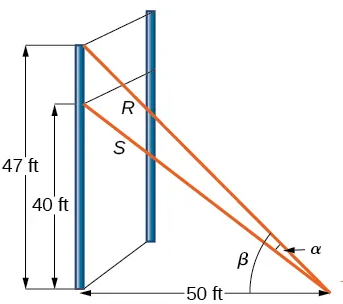
\includegraphics[width=0.35\linewidth]{images/math114_guyWireExample}
    \end{flushleft}
    \vspace*{\stretch{1}}
  \end{ex*}

  \pagebreak
\end{document}
